\documentclass[12pt]{article}
\usepackage{fancyhdr}     % Enhanced control over headers and footers 
\usepackage[T1]{fontenc}  % Font encoding
\usepackage{mathptmx}     % Choose Times font 
\usepackage{microtype}    % Improves line breaks      
\usepackage{setspace}     % Makes the document look like horse manure 
\usepackage{hyperref}
\hypersetup{
	colorlinks   = true, %Colours links instead of ugly boxes
	urlcolor     = blue, %Colour for external hyperlinks
	linkcolor    = black, %Colour of internal links
	citecolor   = black %Colour of citations
}
\usepackage{graphicx}
\usepackage{subcaption}
\usepackage{endnotes}
\usepackage{float}
\usepackage{algorithm}
\usepackage{algpseudocode}
\usepackage{multicol}
\usepackage{tikz}
\usetikzlibrary{snakes}
\usepackage{rotating}

\usepackage[style=apa,backend=biber,citestyle=numeric]{biblatex}
\addbibresource{../refs.bib}

\title{Bayesian Neural Networks}
\author{
	Blair, Taylor
	\and
	Sorgmon, Ava
	\and
	Conor
}
\date{\today}
\let\footnote=\endnote

\usepackage{verbatim}

\pagestyle{fancy} % Default page style 
\lhead{Blair, Sorgman, Conor}
\chead{}
\rhead{\thepage}
\cfoot{}
\rfoot{}
\renewcommand{\headrulewidth}{1pt}
\renewcommand{\footrulewidth}{1pt}
\renewcommand{\theendnote}{\Roman{endnote}} 



\begin{document}
\doublespacing
\maketitle



\begin{abstract}
	Bayesian Neural Networks are...
\end{abstract}

\tableofcontents

\section{Introduction}

\subsection{Neural Networks}


\subsection{Bayesian Neural Networks}

Bayesian Neural were invented by Ralph Merkle. Ralph Merkle initially patented Merkle trees for digital signatures....

\begin{figure}[H]
	\centering
	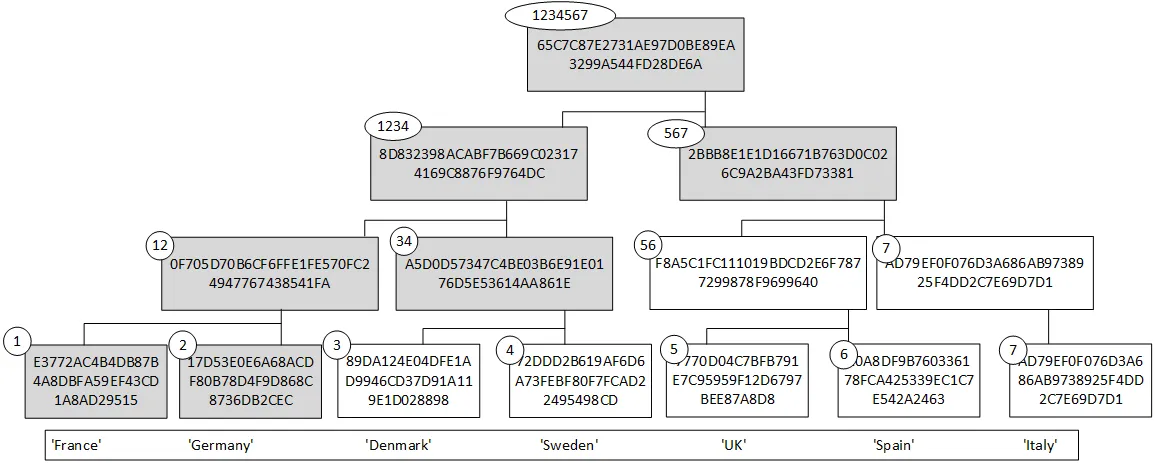
\includegraphics[width=.8\textwidth]{../Images/merkle-example.png}
	\caption{Basic Merkle Tree\cite{wikipedia-merkle-tree}}
\end{figure}


....


\subsection{History}

\begin{figure}[H]
	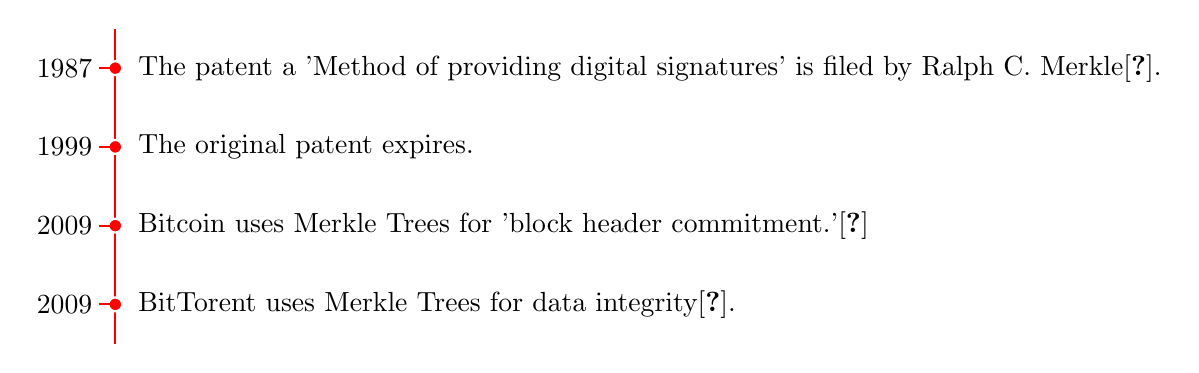
\begin{tikzpicture}[scale=0.5,every node/.style={outer sep=5pt}]
		%Notation: {year, the title of the event}
		%NOTE! Everyting is zero-based
		\def\ourInfo{{
				{"1987"," The patent a 'Method of providing digital signatures' is filed by Ralph C. Merkle\cite{merkle-patent}."},
				{"1999","The original patent expires."},
				{"2009","Bitcoin uses Merkle Trees for 'block header commitment.'\cite{friedenbach_alm_2017}"},			
				{"2009","BitTorent uses Merkle Trees for data integrity\cite{bep30}."},
		}}
		\pgfmathsetmacro{\length}{3}% Zero based.
		
		% Loop through the array containing all events.
		\foreach \i in {0, ..., \length}{
			\pgfmathsetmacro{\year}{\ourInfo[\i][0]}% Get the left cell (year)
			\pgfmathsetmacro{\eventName}{\ourInfo[\i][1]}% Get the right cell (event name)
			\draw[thick,red] (0,-2*\i-2)--(0,-2*\i);% Draw vertical line
			\ifnum \i=0 % Should be in red text
			\draw(0,-2*\i-1) node[black, right, align = left]{\eventName};% Display the event name
			\draw(0,-2*\i-1) node[black, left] {\year};
			\else % Should be in black text
			\draw(0,-2*\i-1) node[right, black]{\eventName};% Display the event name
			\draw(0,-2*\i-1) node[left] {\year};% Display the year
			\fi
		}
		% Draw the bullet with the dash
		\foreach \i in {0, ..., \length}{
			\filldraw[draw = white, fill = red,thick] (0,-2*\i-1) circle (5pt);
			\draw[thick,red] (-12pt,-2*\i-1)--(0,-2*\i-1);
		}
	\end{tikzpicture}
\end{figure}



\section{Literature Review}

Merkle Trees are a component of several projects, as such many papers provide incremental changes towards certain operations on Merkle trees. This paper references the original patent by Ralph Merkle \cite{merkle-patent} in addition to descriptions of Merkle tree operations given by Boneh and Shoup \cite{boneh2020graduate}. As secondary sources, the implementation of Merkle trees in Bitcoin \cite{friedenbach_alm_2017} provides a real example of the impact of hash functions in addition to a whitepaper from the BitTorrent project\cite{bep30}.

\section{Construction}
 Merkle trees are constructed from the bottom up by hashing data as the leaf nodes.
 
 \begin{algorithm}[H]
 	\caption{Merkle tree construction}
 	\begin{algorithmic}
 		\For{$i = 1,\ldots, n$} \Comment{Compute leaf node hashes}
 		\State $y_i \leftarrow h(x_i)$  
 		\EndFor
 		 \For{$j= 1,\ldots, n-1$}  \Comment{Compute intermediate Nodes from $y_{n+1}, \ldots , y_{2n -1}$}
 		\State $y_{i+n} \leftarrow h(y_{2i-1}, y_{2i}) $ \Comment{Hash leaf nodes below for new hash}
 		\EndFor
 		\State \Return $Y$ \Comment{Return tree where $y_{2n-1}$ is the root}
 	\end{algorithmic}
 \end{algorithm}
 
When referring to the parts of a Merkle tree the most common terminology is "root hash" which refers to the hashed value of the root of the tree and "leaf hash" which refers to the hash for a given data block. 



\section{How it works}



\section{Use Cases}

...


\section{Simulation}

We used the Cifar 10....

\section{Closing}





\newpage

\printbibliography


\end{document}
